\chapter{Estado del Arte}

\section{Análisis del Estado del Arte}

Los chatbots son agentes conversacionales que pueden interactuar con los usuarios a través de lenguajes naturales y también pueden describirse con el término más amplio de interfaces de usuario conversacionales (Referencia a PaPer state-of-the-art). El auge de esta tecnología en los últimos años es debido a que puede ser utilizada como mano de obra a un coste menor en una amplia gama de campos, entre ellos pueden destacar la atención al cliente, la asistencia personal o la pedagogía. Y no hay mejor forma de asegurar el potencial de los chatbots que mostrando el aumento de inversión en IA en el campo de las telecomunicaciones (Figura \ref{fig:inversion_chatbot}); y viendo que empresas están apostando por esta tecnología, como pueden ser cinco grandes empresas tecnológicas como son Google, Apple, Facebook, Microsoft y Amazon. Aunque basándonos en este párrafo de la sensación de que todas las empresas deberían disponer de chatbots, esta tecnología necesita de cierta planificación y comprensión de la tecnología, pues requiere de una gran inversión inicial, dado su gran requerimiento de información para funcionar de forma correcta.

\begin{figure}[h]
\centering
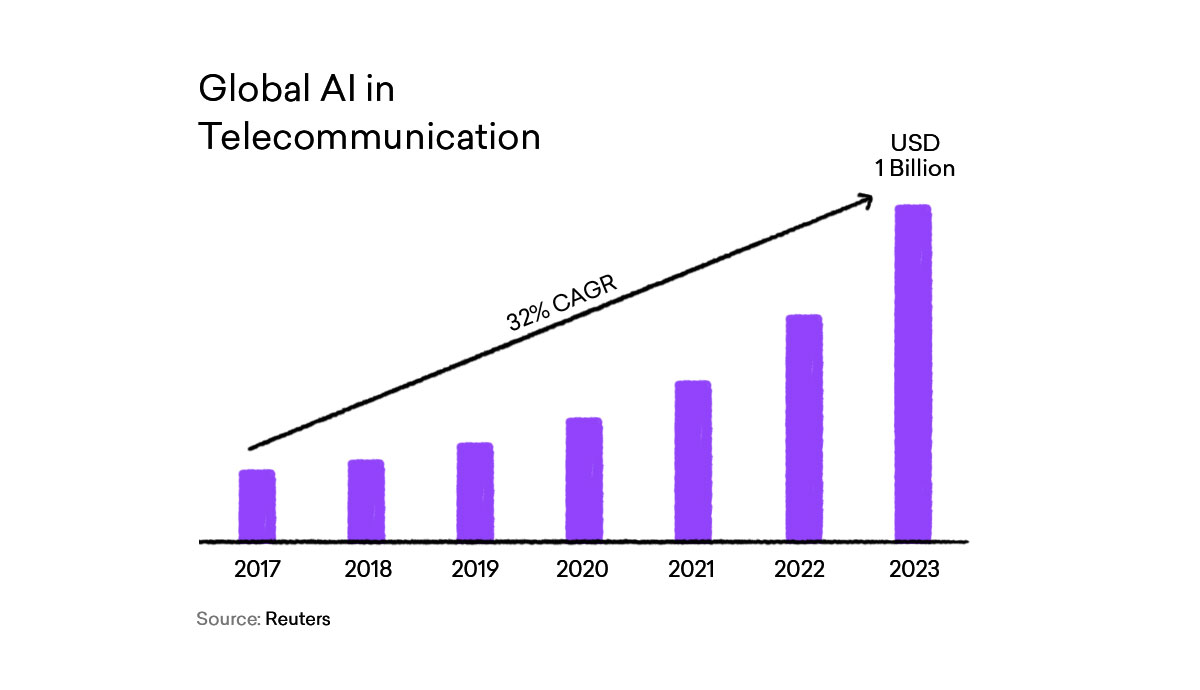
\includegraphics[width=1.0\textwidth]{imagenes/02_EstadoDelArte/inversion_chatbots.jpg}
\begin{center}
Fuente: \url{https://es.aivo.co/blog/chatbots-in-telecom}
\end{center}
\caption{Estimación de la inversión en IA en el campo de las telecomunicaciones}
\label{fig:inversion_chatbot}
\end{figure}

Para personas que están empezando a investigar para comprender los chatbots, se encuentran con la dificultad de la poca claridad de las revisiones bibliográficas existentes dado que adolecen de tres problemas notables (Referencia a PaPer state-of-the-art). En primer lugar, nos encontramos con el problema que aparece nada más empezar, y es la carencia de un esquema de clasificación de chatbots, dado que no se ha definido una clasificación global. La clasificación más extendida es la clasificación según el mecanismo de recuperación y de generación de respuestas, donde destacan los chatbots que hacen uso de bases de conocimientos estáticas, es decir, chatbots basados en reglas; y los chatbots que hacen uso de mecanismos de aprendizaje e inferencia adaptativos, es decir, los chatbots basados en inteligencia artificial. En segundo punto, las revisiones están desactualizadas en el ámbito de la generación de respuestas dado el rápido avance de las técnicas computacionales. En tercer lugar, las revisiones no están muy centradas en la aplicación empresarial de los chatbots ni en su usabilidad, sino que más bien están centradas en el aspecto técnico.

La estructura de los chatbots ha ido evolucionando y extendiéndose. Originalmente, la estructura de los chatbots era la descrita por Abdul-Kader y Woods, donde se podía reconocer tres componentes: interfaz, un clasificador y un graphmaster. Esta estructura está muy desactualizada a día de hoy, ya que en la estructura original la interfaz solo tenía previstas entradas en forma de texto, pero hoy en día las entradas son de tipo multimedia, por lo que es necesario actualizar la interfaz a una interfaz multimedia, y añadir un nuevo componente a la estructura, encargado de manejar esas entradas multimedia y convertirlas en entradas de texto que se puedan manejar para generar respuestas; además dado el auge de los chatbots basado en generación, a día de hoy el componente del graphmaster no tiene sentido, dado que las respuestas se generan utilizando modelos pre entrenados realizando inferencias basándose en las entradas, por lo que tener un manejador para el almacenamiento de conocimiento deja de tener sentido, por lo tanto, en la estructura el graphmaster debe ser actualizado por un modelo generador de respuestas. Sobre la base de todas estas actualizaciones sobre la estructura original de Abdul-Kader y Woods, obtenemos la estructura actual de los chatbots, que se muestra en la Figura \ref{fig:estructura_state_of_art}. Finalmente, tenemos cuatro componentes: la interfaz, un procesador multimedia, un análisis de entrada multimodal y un generador de respuestas.

\begin{figure}[h]
\centering
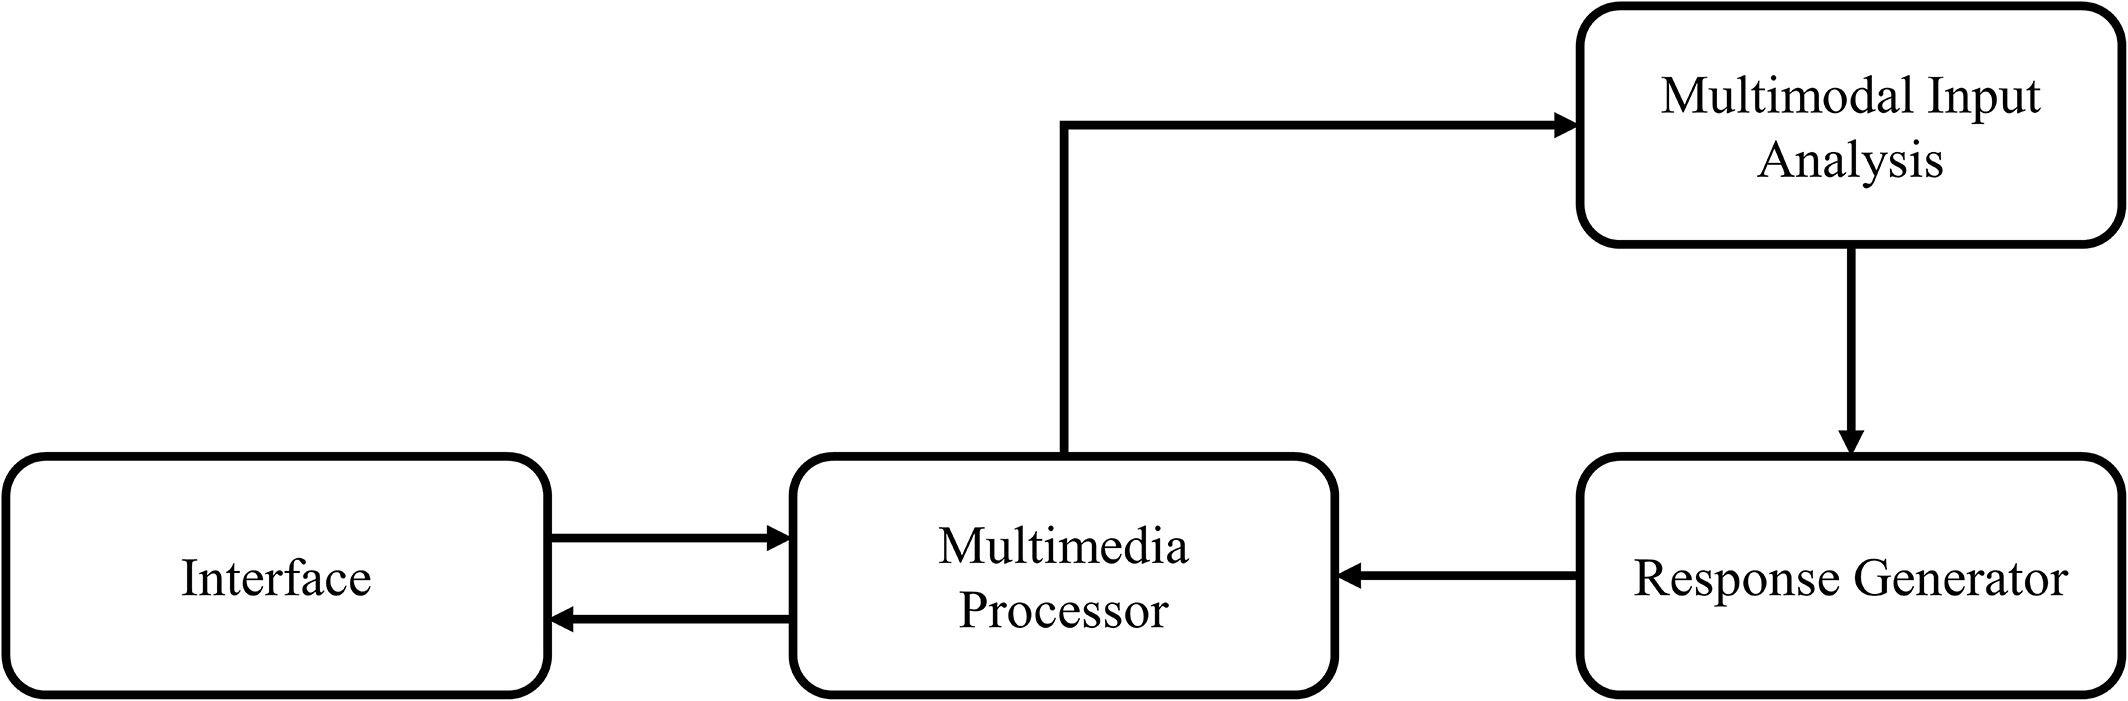
\includegraphics[width=0.8\textwidth]{imagenes/02_EstadoDelArte/estructura_state_of_art.jpg}
\begin{center}
Fuente: A critical review of state-of-the-art chatbot designs and applications (Referencia a PaPer state-of-the-art)
\end{center}
\caption{Estructura de los chatbots actuales}
\label{fig:estructura_state_of_art}
\end{figure}

Un componente que se muestra en la Figura \ref{fig:estructura_state_of_art} y que no se ha mencionado explícitamente cuál es su labor es el análisis de entrada multimodal. Este análisis efectúa un pretratamiento de los datos de entrada, hoy en día se intenta mejorar este componente con técnicas avanzadas de comprensión del lenguaje natural (NLU).

En el caso de los chatbots basados en la recuperación, el generador de respuestas desempeña el mismo papel que el graphmaster, ya que almacena y recupera las respuestas, mientras que en el caso de los chatbots basados en la generación, asigna la entrada normalizada transferida desde la unidad de pretratamiento de la entrada a la salida (Referencia a PaPer state-of-the-art).

Centrándonos en el componente del generador de respuestas, a día de hoy se utilizan distintas técnicas para implementar este componente. Las técnicas más destacadas son las siguientes:

\begin{itemize}
\item \textbf{Template:} Esta técnica se compone de patrones y plantillas formando pares con ellos. Para generar las respuestas se busca el patrón que más concuerde con la entrada recibida, y una vez se haya elegido un patrón se devuelve la plantilla asociada al mismo. El lenguaje que más destaca en esta técnica es AIML \footnote{\url{http://www.aiml.foundation}}. La desventaja de tener que crear los archivos AIML se puede suplir mediante la extracción automática de conocimientos, reduciendo el trabajo manual. Los chatbots basados en plantillas son sencillos de producir, por lo tanto, son una opción popular para chatbots a pequeña escala.
\item \textbf{Corpus:} Son una buena técnica como alternativa a los template cuando se están construyendo chatbots a gran escala, debido a que con los templates al aumentar de escalas aumenta el número de patrones y trae consigo búsquedas más lentas lo que ralentiza la generación de respuestas. Existen dos tipos de chatbots basados en Corpus, un tipo de chatbots basados en corpus que no selecciona cuidadosamente el conocimiento y otro que si lo hace. El tipo que selecciona cuidadosamente el conocimiento se puede implementar mediante bases de datos o mediante modelos de ontología, los modelos de ontología tienen una gestión más flexible del conocimiento que las bases de datos, la generación en este tipo de chatbots se realiza también con búsqueda pero esta vez en las estructuras descritas anteriormente. El tipo que no selecciona cuidadosamente el conocimiento transforma las palabras en vectores que representan los significados semánticos de las palabras en un espacio multidimensional, la generación en este tipo de chatbots se realiza mediante el cálculo de la distancia entre los pares de entrada del usuario y de consulta-respuesta, se empareja la consulta con la menor distancia y se selecciona su correspondiente respuesta como salida. Debido a la gran capacidad de gestión del conocimiento, varias aplicaciones que requieren un conocimiento formal del dominio utilizan chatbots basados en corpus (Referencia a PaPer state-of-the-art).
\item \textbf{Intent:} Los chatbots basados en intenciones se emplean ampliamente para los sistemas orientados a tareas que presentan diálogos de varios turnos (Referencia a PaPer state-of-the-art). En el caso de esta técnica es necesario añadir adicionalmente un componente de análisis de entrada multimodal (SLU), dentro de él se efectúa un análisis semántico de las entradas, para este análisis se suelen usar técnicas avanzadas de NLU, además a partir del análisis semántico realiza una clasificación para saber a qué intención pertenece la entrada mediante técnicas de aprendizaje automático. Dado que estos chatbots están orientados a tareas es necesario tener dentro de la generación de respuestas técnicas de DST para la identificación del estado del diálogo, y técnicas de DPO para el procesamiento del estado del diálogo; estas dos técnicas son necesarias para establecer la secuencia de los diálogos. Las bases de conocimiento de los generadores de respuestas en los chatbots basados en intenciones están compuestas principalmente de frases de entrenamiento, intenciones y respuestas. Para generar las respuestas se analiza semánticamente las entradas en el módulo SLU, posteriormente se utiliza el módulo DST para estimar el estado de los diálogos actuales y finalmente se utiliza el módulo DPO para determinar las acciones y respuestas. Este tipo de chatbots son empleados por grandes empresas como puede ser Google con Dialogflow \footnote{\url{https://dialogflow.cloud.google.com}} (originalmente llamado Api.ai) o también existen alternativas de código abierto como puede ser Rasa \footnote{\url{https://rasa.com/}}.
\item \textbf{Red neuronal recurrente (RNN):} Los chatbots creados con esta técnica dejarán de estar basados en la recuperación, como pasaba en las tres anteriores técnicas, si no que estarán basados en la generación, pero esto que quiere decir, en definitiva quiere decir que la generación de las respuestas no se realizará mediante búsquedas en alguna estructura y sustitución mediante pares consulta-respuesta. La generación de las respuestas se efectúa mediante inferencias con modelo de redes neuronales recurrentes. Estos chatbots, a diferencia de los chatbots basados en intenciones, no están orientados a las tareas y esto deriva del problema que conllevan las redes neuronales, y no es otro que las redes convierten al chatbot en una caja negra, esto quiere decir que la respuesta del chatbot ante cierta entrada es incierta incluso para su creador, este inconveniente se convierte en una ventaja si orientamos a los chatbots al chat, dado que esta incertidumbre en la respuesta da una gran sensación de naturalidad y creatividad durante la conversación, por lo que son apropiados para actividades relacionadas con el entretenimiento y la salud mental. Estos chatbots se han visto muy potenciados en los últimos años debido al rápido desarrollo del aprendizaje profundo. Uno de los mayores hitos en el aprendizaje profundo ha sido la creación de GPT-3 \footnote{\url{https://openai.com/blog/openai-api}}, el cual es un nuevo modelo de inteligencia artificial que permite generar lenguaje escrito creado por la empresa OpenAI. Como se ha mencionado anteriormente ya no se realiza recuperación para la generación de respuestas, por lo tanto, las bases de conocimiento de los chatbots basados en RNN estarán compuestas de los conjuntos de datos de entrenamiento. El resultado de los chatbots basados en la generación depende de la especificación del modelo, los conjuntos de datos de entrenamiento, el proceso de entrenamiento y la entrada del usuario (Referencia a PaPer state-of-the-art).
\item \textbf{Aprendizaje por refuerzo (RL):} Este tipo de chatbots suelen estar basados en la recuperación y utilizan plenamente el contexto de entrada para la búsqueda de respuestas óptimas (Referencia a PaPer state-of-the-art). Dado que se basan en la recuperación, en sus bases de conocimientos hay pares de consulta-respuesta predefinidos. El método RL se basa principalmente en el proceso de decisión de Markov. Al igual que pasaba en los chatbots basados en templates, en los chatbots basados en RL se utlizan representaciones vectoriales, en concreto el estado del chatbot es una representación vectorial de un turno de conversación. Este vector puede contener la respuesta derivada de la entrada o adicionalmente puede contener el acto de diálogo, el sentimiento del usuario y el enunciado genérico del usuario. El contexto de la comunicación forma una secuencia de estados. Aunque es una técnica basada en la recuperación, esta recuperación es distinta a la descrita en las anteriores técnicas, en el caso de esta técnica se utiliza una política para encontrar la respuesta adecuada, esta política debe ser bien entrenada para lo que son necesarios diálogos predefinidos. Este tipo de chatbots se pueden usar para secciones de "Preguntas frecuentes".
\item \textbf{Enfoques híbridos:} El intento de combinar varias técnicas para suplir las desventajas de ambas con las ventajas de cada técnica es algo que se ha intentado en una multitud de ámbitos, y este no iba a ser menos. En el paper (Referencia a PaPer state-of-the-art) se hace referencia a una serie de propuestas de diferentes investigadores. Una de ellas puede ser la propuesta por Li Wu y Wu Wu propusieron un marco de correspondencia secuencial basado en una RNN. El marco considera las relaciones entre los enunciados anteriores y las respuestas candidatas y selecciona las respuestas óptimas para el contexto.
\end{itemize}

Si nos fijamos en la técnica utilizada para crear el chatbot podemos obtener una buena clasificación de los mismos.

Una vez estudiada la estructura actual de los chatbots. A continuación voy a exponer algunas de las posibles aplicaciones que pueden tener los distintos chatbots.

La primera aplicación y puede que la más usada por la gente en general es la atención al cliente para el comercio electrónico. Dado el gran crecimiento de sector, se ha producido un elevado aumento de la carga de trabajo. Como se ha indicado anteriormente, por ejemplo en el caso de los chatbots basados en intenciones, los chatbots son capaces de reducir la carga de trabajo y consecuentemente también reduce los costes humanos. La calidad del servicio proporcionado por estos chatbots está en continua mejora debido a la dificultad de manejar peticiones muy complejas por parte del usuario y otros problemas como el amplio dominio necesario para contestar de forma correcta durante toda la conversación y no solamente para contestar, sino también para realizar un servicio agradable para el usuario.

La siguiente aplicación a exponer también está muy extendida y es utilizada asiduamente por multitud de personas. Los chatbots de asistencia personal pueden emplearse para aumentar la eficiencia del trabajo o para gestionar la vida cotidiana del usuario. Un posible ejemplo podría ser Siri \footnote{\url{https://www.apple.com/es/siri}}, que es un chatbot incorporado en todos los dispositivos iPhone.

Otra posible aplicación de los chatbots es la asistencia sanitaria. Esta clase de chatbots actúan como asistentes médicos para el diagnóstico de enfermedades. La comprensión de los síntomas del paciente es primordial en el proceso de detección de la enfermedad, y una de las principales funciones de estos chatbots es recoger suficiente información de los pacientes (Referencia a PaPer state-of-the-art). Aunque en los aspectos médicos la última palabra la tiene un profesional humano, los chatbots puede realizar diagnósticos previos rápidamente dada su inmenso conocimiento al que se puede acceder en un instante, cosa que no sucede con los humanos lo que ralentiza el diagnóstico. Esta enorme base de conocimiento es muy importante en la medicina debido al vasto dominio de este campo.

Y como última aplicación a exponer tenemos los agentes conversacionales pedagógicos. Estos chatbots están diseñados para ayudar al aprendizaje. Dado que la función principal de los chatbots es comunicarse con los usuarios, el aprendizaje de idiomas ha sido una de las principales vías perseguidas (Referencia a PaPer state-of-the-art), ya que el aprendizaje de idiomas está a la orden del día de todo el mundo. Estos chatbots son útiles para enseñar a usuarios mediante conocimientos de expertos, sin que sea necesario una ingente cantidad de expertos para enseñar, puesto que esta cantidad de expertos en ciertos campos y lugares no está disponible.

En todas estas aplicaciones existe el problema de la seguridad de los datos necesarios por el chatbot, este aspecto está muy presente en los últimos años debido a los múltiples casos publicados sobre falta de seguridad con los datos de los usuarios. De cara al futuro se pretende que aumente la seguridad de estos datos.

Llegados a este punto en el que ya hemos analizado el estado actual de los chatbots, únicamente nos queda analizar cuál es la dirección de las futuras investigaciones en este sector. Estas investigaciones estarán centradas en paliar las deficiencias actuales y en mejorar aún más las capacidades actuales.

Uno de los principales problemas de los chatbots es la ingente cantidad de datos que necesitan para empezar a funcionar. Actualmente, este conocimiento es almacenado en estructura de distinto tipo, sin tener un esquema unificado. Esta variedad de bases de conocimiento distintas dificulta la creación de nuevos chatbots al no poder reutilizar datos utilizados en chatbots anteriores. Una posible futura mejora sería la estandarización de la gestión del conocimiento para poder realizar esta transferencia de datos entre chatbots de forma eficiente.

Un aspecto analizado anteriormente es la generación de las respuestas, este aspecto aunque ha sufrido un gran desarrollo en los últimos años, todavía no ha llegado a alcanzar su máximo nivel, esto se puede comprobar simplemente con ver, tal y como indica el paper (Referencia a PaPer state-of-the-art), que todavía nadie ha ganado el premio de oro del Premio Loebner, el concurso de pruebas Turing más famoso en el ámbito de los chatbots. Las futuras investigaciones están orientadas a la mejora de las técnicas de aprendizaje profundo. Estas técnicas son entre otras las redes generativas adversativas (GAN), este tipo de redes está muy extendido en el mundo de la visión por computador, pero todavía no se ha llegado a conseguir una integración de esta técnica en el mundo de los chatbots.

Un aspecto de los chatbots que todavía tiene mucho potencial por explotar es sin duda la interfaz. Hasta ahora solamente hemos indicado que se están utilizando interfaces multimodales. Pero no se está sacando todo el partido a este tipo de interfaces, dado que actualmente únicamente se realiza una conversión de todo tipo de entradas a una entrada en formato de texto. Pero las entradas multimodales contienen información adicional a la que se extrae hoy en día, como puede ser el lenguaje no verbal durante una conversación por voz. Este lenguaje no verbal proporciona mucha información que puede ayudar a la generación de respuesta y a tener un mejor contexto de la conversación. Para que toda esta información no se desperdicie se debe avanzar en la investigación para la extracción de esta información. Otro aspecto de la interfaz donde es necesaria la investigación es la devolución de la respuesta a través de la interfaz, ya que hasta ahora estábamos hablando de como se debía mejorar la entrada de información en la interfaz. La devolución de esta información se puede efectuar de muchas maneras, escrita, por voz, etc. Lo verdaderamente importante en la devolución de la respuesta es que el usuario perciba esa respuesta con facilidad, con una buena estética que atraiga la atención del mismo. Una de las líneas de futuras investigaciones son los avatares 3D, es decir, la respuesta es devuelta por voz, pero lleva añadida la gesticulación de un avatar 3D.

Una dirección en la que se pueden realizar futuras investigaciones son las aplicaciones del chatbot. Dado el auge del internet de las cosas (IoT) hoy en día hay todo un campo donde integrar los chatbots para mejorar el servicio a los usuarios, como pueden ser los coches inteligentes, los hogares inteligentes, y muchos más.

Por último, tal y como se ha indicado anteriormente, uno de los grandes problemas actualmente de los chatbots es la falta de seguridad con los datos, este es un aspecto crucial en todas las futuras investigaciones.

\section{Herramientas para el desarrollo del chatbot}

Un aspecto a tener en cuenta a la hora de elegir una plataforma para desarrollar un chatbot es que existen dos elementos en esta creación.

\begin{itemize}
    \item \textbf{Bot Frameworks}: son las plataformas encargadas de la creación y el alojamiento de los chatbots.
    \item \textbf{Bot Platforms}: son los entornos y aplicaciones donde van a ser desplegados los chatbots para su uso por parte de los usuarios.
\end{itemize}

A la hora de elegir la plataforma donde desarrollar el chatbot habrá que tener en cuenta que tanto el Bot Framework como el Bot Platform elegidos se adecuan a los requisitos del chatbot a crear.

Una posible clasificación de las plataformas puede ser en base al modo de creación de los chatbots. Dentro de esta clasificación encontramos las siguientes plataformas:

\begin{itemize}
    \item \textbf{Plataformas visuales}
    \item \textbf{Plataformas conversacionales}
    \item \textbf{Plataformas programables}
\end{itemize}

\subsubsection*{Plataformas visuales}

En estas plataformas no es necesario tener conocimientos técnicos para crear un chatbot. Por esta razón son las plataformas ideales para personas que no tienen conocimientos en programación ó IA. Algunos ejemplos de este tipo de plataformas pueden ser: Chatfuel y Octane AI. Esta simpleza en la creación del chatbot afecta en la posible complejidad que pueda tener el chatbot, por lo tanto no son las mejor opción para chatbots con con algo de complejidad, pero si para chatbots muy simples.

\subsubsection*{Plataformas conversacionales}

En estas plataforma es posible la creación de chatbots algo más complejos que en las plataformas visuales. Estos chatbots son capaces de mantener una conversación con un usuario, pero que a diferencia de los anteriores chatbots esta conversación no tiene un objetivo específico. Un posible ejemplo de este tipo de plataformas puede ser AIML, aunque AIML no es en sí una plataforma sino más bien un lenguaje de programación, si se convierte en una plataforma si se combina el lenguaje con alguna plataforma donde se permita al menos el alojamiento del chatbot. Este tipo de plataformas ya no está orientado a usuarios sin conocimientos técnicos, sino más bien a usuarios que tengan cierto nivel técnico y que busquen crear chatbots con cierta complejidad. 

\subsubsection*{Plataformas programables}

En estas plataforma se pueden crear desde los chatbots más simples hasta los más complejos. Para poder aumentar la complejidad se hace uso de técnicas de IA junto a las técnicas que ya se utilizaban en las anteriores plataformas, y aumenta la posibilidad de interactuar con servicios externos a la plataforma como pueden ser bases de datos y muchos más servicios. Algunos ejemplos de este tipo de plataformas pueden ser: Google Dialogflow, Microsoft Bot Framework y IBM Watson. \newline\newline


En la actualidad se dispone de un número elevado de plataformas capaces de crear chatbots de diferentes complejidades. De entre este número elevado de plataforma he seleccionado unas cuantas para analizarlas en detalle como posibles plataformas donde crear mi chatbot. En esta lista de plataformas no se encuentra ninguna plataforma visual dado que no posibilitan la complejidad necesaria para crear mi chatbot.


\subsection{AIML}

\subsubsection*{Información general}

El lenguaje de programación AIML (Artificial Intelligence Markup Language) fue desarrollado por el doctor Richard Wallace y la comunidad de código abierto Alicebot en la segunda mitad de los años 90. AIML es un lenguaje basado en etiquetas, al igual que los lenguajes HTML y XML. En concreto el lenguaje AIML se baso en gran medida en el lenguaje XML. Este parecido entre lenguajes no es una casualidad, si nos fijamos en el entorno de la época en la que se desarrollo AIML. A finales de la década de 1990 se produjo la explosión de la World Wide Web. Esta explosión trajo consigo al lenguaje HTML, que surgió como un lenguaje simple que sirviese como estándar para la creación de páginas web. El objetivo de HTML era que cualquier persona con pocos conocimientos informáticos fuese capaz de crear una página web. Esta filosofía de estándar de una tecnología y de simpleza la tomaron como ejemplo los creadores de AIML durante su desarrollo, intentando que AIML se convirtiese en un estándar en la creación de chatbots y que además fuese accesible al mayor número de usuarios. Además del lenguaje HTML, durante la década de 1990 se creo el lenguaje XML, que también se convirtió en un estándar.

Actualmente, al igual que le ha pasado al lenguaje HTML, el lenguaje AIML se ha ido actualizando con el tiempo añadiendo le nuevas funcionalidades que permitiesen crear chatbots más complejos, acorde al incremento de requisitos en los chatbots que ha ido surgiendo con el paso de los años. En el momento de la realización de este TFG, la última versión publicada de AIML es la versión 2.1 . Al crear agentes conversacionales con AIML, estos agentes no se convierten en cajas negras por lo tanto son más transparentes al programador que los creados con otras plataformas más grandes, ya que con AIML se crean chatbots basados en reglas. AIML se puede escribir en casi cualquier lenguaje natural.



→ http://www.aiml.foundation

\subsubsection*{Uso}

Para crear un chatbot con AIML es necesario generar una serie de archivos, que contendrán el estado y la configuración del bot.

En el estado del chatbot podemos distinguir el estado del bot y el estado del cliente. El estado del bot se define usando valores globales para las propiedades del bot, cada bot tendrá sus propiedades. El estado del cliente se define usando variables locales, cada cliente tendrá su estado específico.

La configuración del bot se define en los archivos AIML, en los archivos Learnf, en los Sets y en los Maps. Dentro de los archivos AIML se define la lógica del chatbot a base de añadir reglas, además en estos archivos se pueden realizar conexiones con otros chatbots definidos por otra serie de archivos. Dentro de los archivos Learnf se guardan las categorías aprendidas por el chatbot cuando en un template AIML se activa una etiqueta. Las categorías parendidas son globales a todos los clientes del chatbot. Dentro de los archivos Set se define un conjunto de cadenas. Dentro de los archivos Map se define un mapeo de cadena a cadena.

Según el estándar de AIML, esta serie de archivos se pueden definir dónde y cómo quiera el creador del chatbot.

Dado que AIML es sólo un lenguaje de programación, es necesario un framework para la creación del agente conversacional, como pueden ser algunos intérpretes y bibliotecas de código abierto (Python, Node JS, Java) ó servicios web (Pandorabots).

Si se elige la opción de usar intérpretes y bibliotecas de código abierto disponemos de las siguientes posibilidades:

\begin{itemize}
    \item Python $\rightarrow$ Program-Y
    \item Node JS $\rightarrow$ aimlinterpreter
    \item Java $\rightarrow$ Program AB
\end{itemize}

Si se elige la opción de usar servicios web como Pandorabots, uno de los más populares actualmente, se podrá alojar el chatbot en la plataforma y se podrá hacer uso de todas sus funcionalidades. Si nos centramos en Pandorabots disponemos de un editor de AIML, un editor de interfaces, control de versiones a través de Github, chatlogs, conversor de texto a voz y viceversa, posiblidad de añadir un personaje 3D como interación con el chatbot, integración con RESTful APIs y muchos más, según se indica en su página oficial \cite{RefWorks:RefID:14-pandorabots:}.

Muchas de estas funcionalidades depende del tipo de cuenta que se disponga en Pandorabots.

\newpage

\begin{figure}[h]
    \centering
    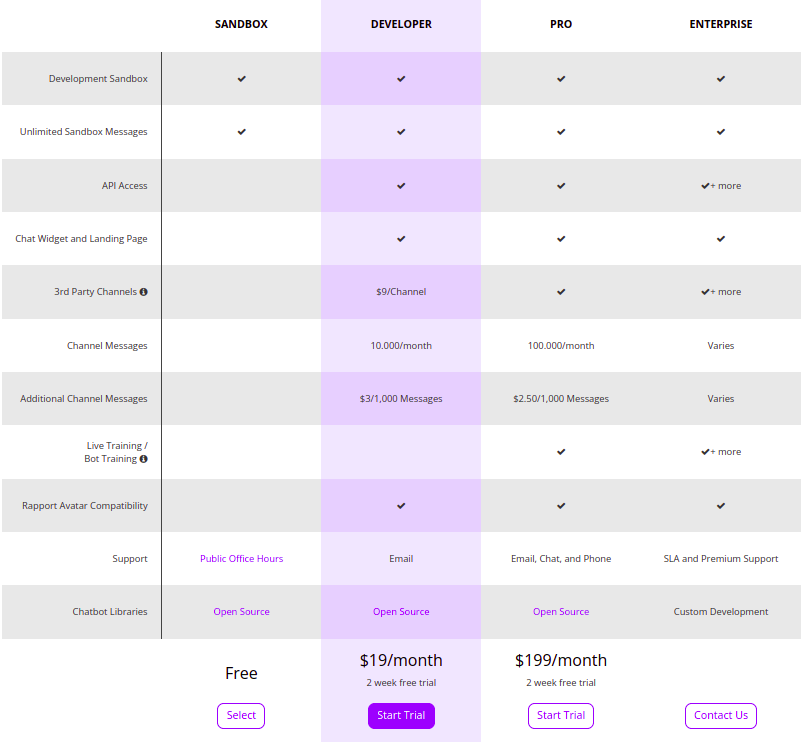
\includegraphics[width=1.0\textwidth]{imagenes/02_EstadoDelArte/cuentas_pandorabots.png}
    \begin{center}
        Fuente: \url{https://developer.pandorabots.com/home.html}
    \end{center}
    \caption{Cuentas disponibles en Pandorabots}
    \label{fig:cuenta_pandorabots}
\end{figure}

En la figura \ref{fig:cuenta_pandorabots} podemos comprobar como con la cuenta gratuita no disponemos de todas las funcionalidad anteriormente descritas.


→ https://developer.pandorabots.com/


\subsubsection*{Extensibilidad}

Dado que hay muchos frameworks para la creación de un chatbot con AIML, dependerá del framework elegido la cantidad de posiblidades de conexiones con APIs o servicios externos al chatbot. 

Para que AIML sea flexible y extensible dispone de la posibilidad de integrar sus propias API's, bases de datos ó también se pueden crear etiquetas propias; pero para ello se debe tener cierto nivel con el lenguaje de programación AIML.

Si optamos por servicios web como Pandorabots para poder disponer de conexión con servicios externos al servicio web o con APIs se debe disponer de una cuenta de pago, no basta con la versión gratuita de Pandorabots.

\subsubsection*{Integración}

Si optamos por servicios web como Pandorabots, al igual que pasa con la extensibilidad, será necesaria una cuenta de pago para poder integrar nuestro chatbot en plataformas de mensajería como Facebook Messenger, Twitter, Telegram y muchos más.

Pero si optamos por framework de código abierto hay una multitud de posibilidades, tantas como nivel de conocimientos tenga el creador del chatbot. Un ejemplo puede ser con Node JS, donde podríamos desplegar el chatbot en cualquier página web a través de una interfaz web que enviase peticiones al servidor creado con Node JS que aloja al chatbot.

\subsubsection*{Ejemplos}

Algunos ejemplos de chatbot implementados con AIML son los siguientes:

\begin{itemize}
    \item \textbf{Rosie}. Chatbot base basado en ALICE 2.0 \footnote{\url{https://github.com/pandorabots/rosie}}
    \item \textbf{Programa-Y}. Chatbot basaso en Python 3.x y AIML 2.0 \footnote{\url{https://github.com/keiffster/program-y}}
    \item \textbf{Cathy}. Chatbot para Discord basado en Python 3 y AIML \footnote{\url{https://github.com/DevDungeon/Cathy}}
\end{itemize}


\subsection{IBM Watson}

\subsubsection*{Información general}

IBM Watson es un portfolio de IBM de aplicaciones, herramientas y soluciones preparadas para la empresa, diseñado para reducir los costes y los obstáculos de IA, además de optimizar los resultados y el uso responsable de la IA según se indica en su página oficial \cite{RefWorks:RefID:15-2021ibm}. Aunque en un inicio IBM Watson no era lo que es ahora actualmente y tampoco se buscaba llegar a este punto. Originalmente IBM Watson surgío como el siguiente gran desafío de la empresa IBM, tras haber salido victorioso de otros grandes desafíos como la victoria de Deep Blue contra Garry Kasparov y el desafío de la supercomputadora Blue Gene. El objetivo que perseguía en sus orígenes Watson era conseguir ganar a competidores humanos en el concurso Jeopardy. Este concurso de televisión estadounidense consistía en un concurso de preguntas sobro una multitud de temas, y los concursantes deberán resolver las preguntas de cada prueba realizando preguntas sobre las pistas que va dando el presentador. Las reglas del concurso obligan a que Watson no sólo sepa conocimientos sobre los temas que se utilizan en el concurso, sino también ha saber realizar preguntas al presentador en base a sus pistas, y además saber distinguir cuando la pista del presentador no es cierta. Todas estos requisitos convierten el ganar este concurso en un gran desafío, la empresa IBM se embarco en este proyecto a mediados de la década del 2000. Finalmente en el año 2011 se llegó a un acuerdo para la realización del programa, donde compitieron dos grandes exconcursantes del programa como son Ken Jennings y Brad Rutter contra Watson. Tal y como se indica en el articulo \cite{RefWorks:RefID:16-best2013ibm}, Watson ganó el juego con \$77,147 , dejando a Rutter y Jennings con \$21,600 y \$24,000 respectivamente.

Tras la victoria de IBM Watson, se empezó a enfocar y rediseñar a Watson hacia distintos sectores como la medicina, la banca ó los agentes conversacionales entre otras. Los agentes conversacionales es el sector que nos interesa investigar.

Dado que IBM Watson está orientado al mundo empresarial destaca por su confianza, es decir, Watson es transparente en cuanto a las decisiones basadas en IA; también protege la privacidad de los datos y su seguridad. Todas estas características son muy valoradas en cualquier producto empresarial, incluso algunas son imprescindibles.

Otro característica de Watson es su procesamiento del lenguaje natural. Al igual que AIML es multilenguaje, pero Watson lo lleva a un aspecto más complejo añadiendo la capacidad de analizar datos complejos y no estructurados, como pueden ser códigos de programación ó incluso formas de expresión específicas de una modalidad de trabajo. Este procesamiento del lenguaje natural no es algo alcanzable por cualquier empresa. La IA de Watson sabe desenvolverse en la situaciones más complejas, como pueden ser situaciones en las que no pueda responder, reenviando la solicitud a un agente humano o hacia algún documento de ayuda; evitando realizar preguntas redundante facilitando la comunicación y haciéndola más natural; y por última sabe manejar solicitudes ambiguas comunes en la comunicación como pueden ser errores ortográficos, cambios de tema, y muchas más situaciones que pueden ser inesperadas para el chatbot en una conversación. Además IBM Watson intenta mejorar su rendimiento aportando al creador del chatbot información sobre que nuevos temas añadir para mejorar la respuesta a las solicitudes.

Y por último destaca que Watson trabaja con cualquier servicio en la nube, lo que facilita su integración en las empresas, ya que no será un impedimento el lugar donde residan los datos de la empresa. Y además el trabajar en cloud facilitará el trabajo con los datos.

En concreto en la página oficial de IBM Watson Assistant \cite{RefWorks:RefID:17-ibm} se destaca la rentabilidad del producto, de hasta un 337\% según el Informe TEI de Forrester \cite{RefWorks:RefID:8-iles2020el}; su precisión, de hasta un 14,7\% superior que las soluciones de la competencia según un reciente estudio publicado sobre machine learning \cite{RefWorks:RefID:18-2020watson}; y su fiabilidad, ya que Watson tiene más de 1000 despliegues de clientes en todos los sectores.



→ https://www.ibm.com/es-es/watson

→ El Total Economic Impact™ de IBM Watson Assistant

→ https://www.ibm.com/es-es/products/watson-assistant

→ https://www.techrepublic.com/article/ibm-watson-the-inside-story-of-how-the-jeopardy-winning-supercomputer-was-born-and-what-it-wants-to-do-next/

→ https://www.ibm.com/blogs/watson/2020/12/watson-assistant-improves-intent-detection-accuracy-leads-against-ai-vendors-cited-in-published-study/

\subsubsection*{Uso}

IBM Watson está pensado para ser utilizado por cualquier persona, da igual que no tenga conocimientos en programación. La creación del chatbot se basa en un editor de arrastrar y soltar. Este editor evita la complejidad de la programación de un chatbot y los posibles errores derivados de esa necesidad de escribir el código en su creación ó en alguna modificación que necesite el chatbot. Es posible crear un chatbot sin escribir una sola línea de código.

\begin{figure}[h]
    \centering
    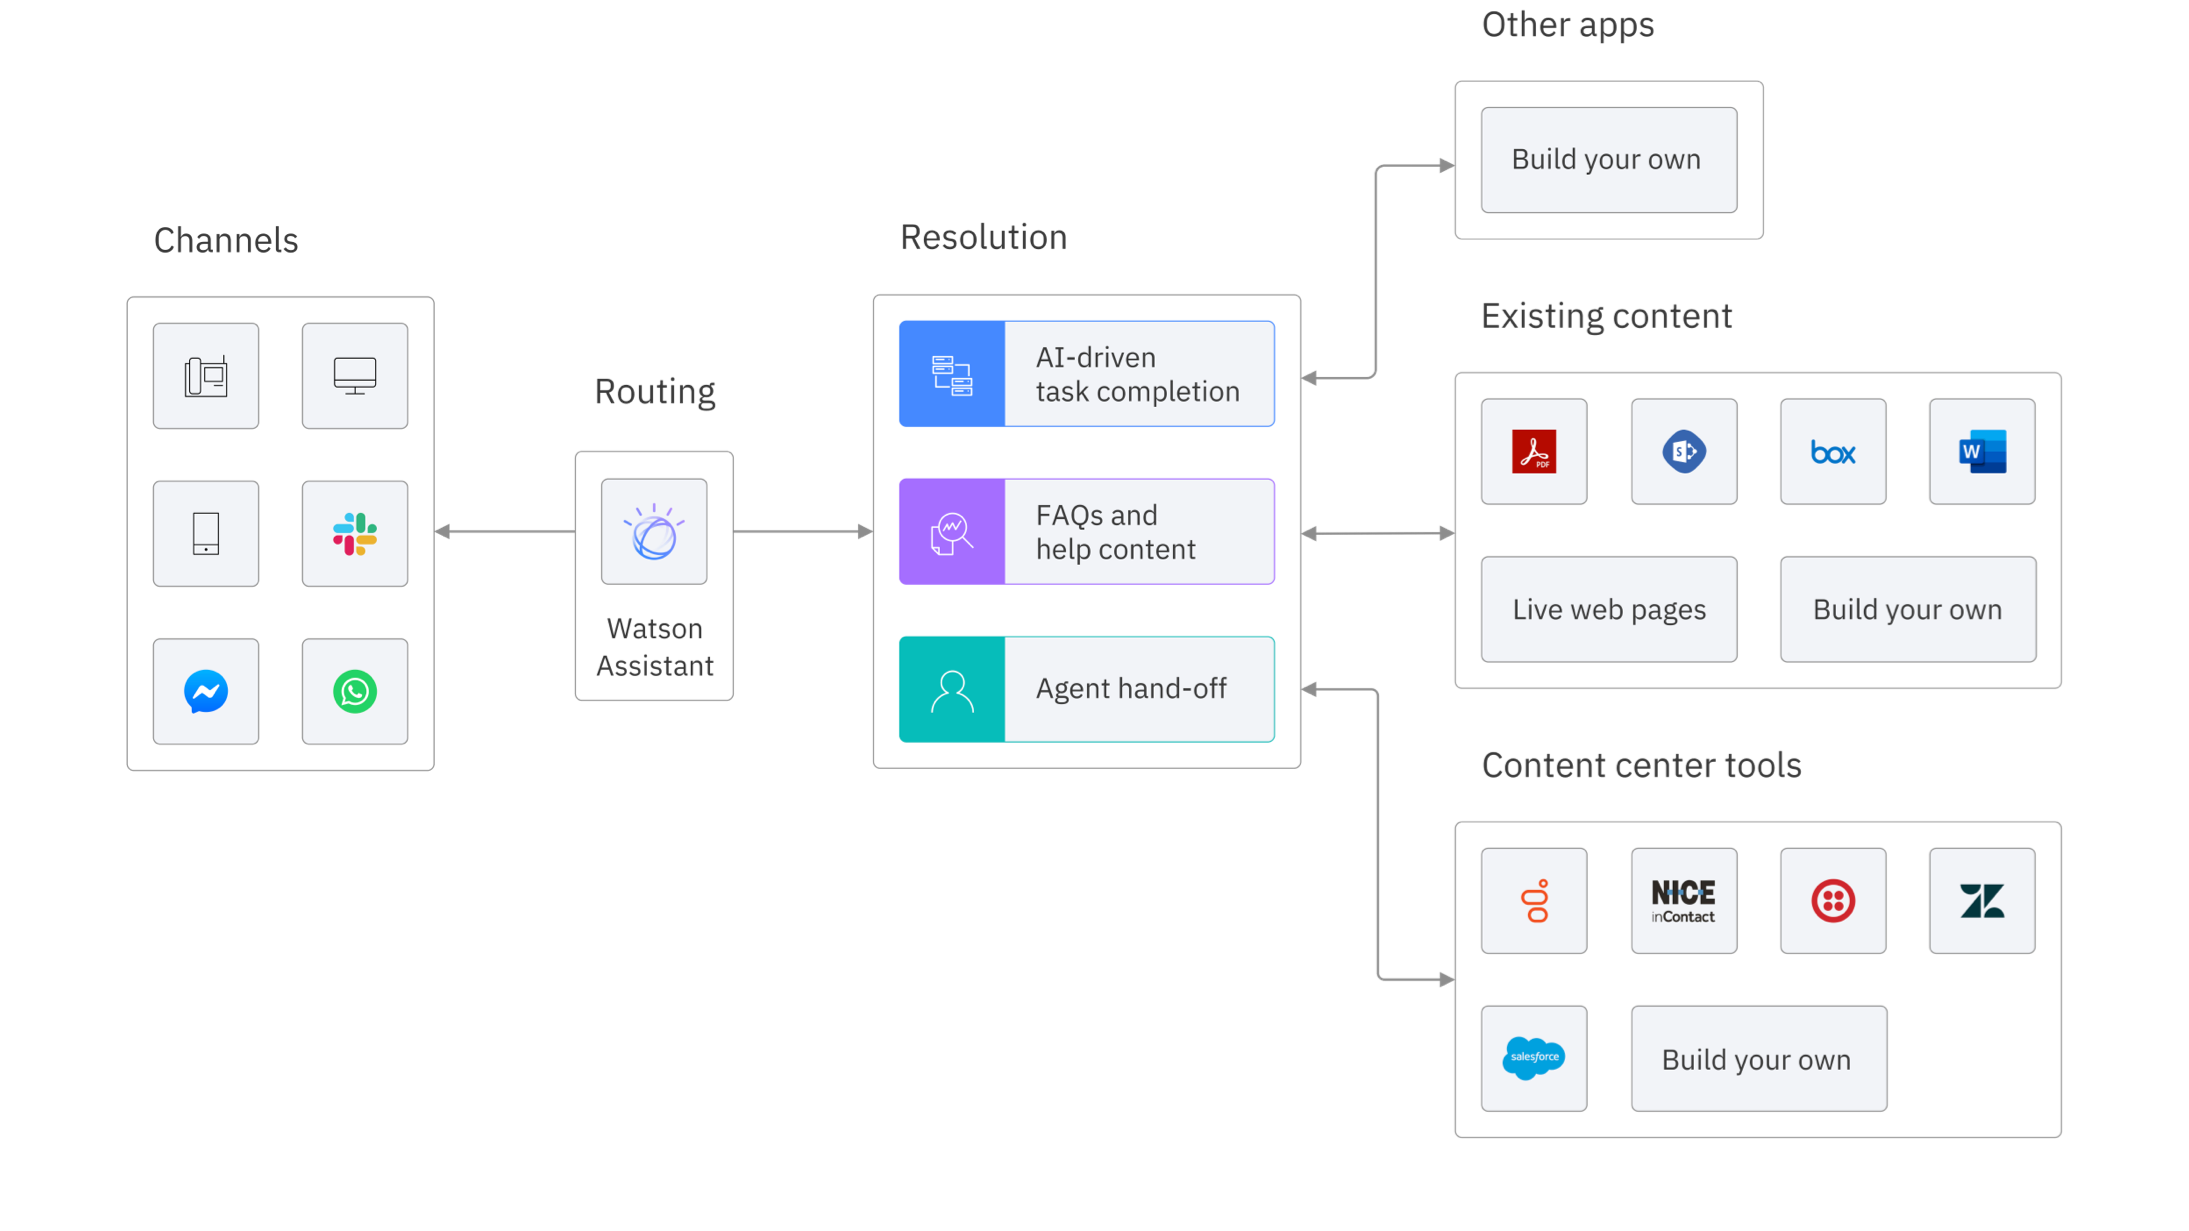
\includegraphics[width=1.0\textwidth]{imagenes/02_EstadoDelArte/editor_IBM_Watson.png}
    \begin{center}
        Fuente: \url{https://www.ibm.com/es-es/products/watson-assistant}
    \end{center}
    \caption{Editor de IBM Watson}
\end{figure}

La IA del chatbot es capaz de comprender un tema en cualquier lenguaje natural con unas pocas frases facilitando la adaptación del chatbot a la funcionalidad que se le quiera dar, adaptándose de forma rápida y precisa al dominio del proyecto.

\subsubsection*{Extensibilidad}

Como se ha indicado en apartados anteriores, IBM Watson es un portfolio de IBM de aplicaciones. En su página oficial \cite{RefWorks:RefID:19-2021productos} se indican las siguientes aplicaciones con las que se puede integrar el chatbot:

\begin{itemize}
    \item IBM Watson Discovery
    \item IBM Watson Natural Language Understanding
    \item IBM Watson Speech to Text
    \item IBM Watson Text to Speech
    \item IBM Watson Knowledge Studio
    \item IBM Watson Language Translator
    \item IBM Watson Natural Language Classifier
\end{itemize}

Entre estas aplicaciones se encuentran algunas muy útiles como IBM Watson Discovery para la extracción y búsqueda de información, IBM Watson Speech to Text para transformar la voz a texto escrito gracias a una potente tecnología de machine learning, IBM Watson Language Translator para traducir dinámicamente información, ó IBM Watson Knowledge Studio para enseñar a Watson el idioma del domino del chatbot.



→ https://www.ibm.com/es-es/watson/products-services

\subsubsection*{Integración}

El chatbot se puede integrar como un chat web, como contestador de llamadas de teléfono ó como un chatbot en una aplicación de mensajería como WhatsApp, Facebook Messenger, SMS y muchos más. Todas estas formas de integrar el chatbot son muy fáciles de realizar.

\subsubsection*{Ejemplos}

Algunos ejemplos de chatbot implementados con Watson son los siguientes:

\begin{itemize}
    \item \textbf{Nanci. Chatbot desarrollado por la empresa GM Financial} \footnote{\url{https://www.gmfinancial.com/en-us/company/newsroom/chatbot.html}}
    \item \textbf{Chatbot desarrollado por la empresa Bradesco} \footnote{\url{https://www.ibm.com/watson/stories/bradesco}}
    \item \textbf{CARL. Chatbot desarrollado por la empresa Siemens} \footnote{\url{https://www.ibm.com/es-es/products/watson-assistant/client-stories}}
    \item \textbf{Chatbot desarrollado por la empresa Humana} \footnote{\url{https://www.ibm.com/watson/stories/humana}}
\end{itemize}




→ https://www.ibm.com/watson/stories/humana
→ https://www.ibm.com/es-es/products/watson-assistant/client-stories
→ https://www.ibm.com/watson/stories/bradesco
→ https://www.gmfinancial.com/en-us/company/newsroom/chatbot.html


\subsection{Google Dialogflow}\label{subsec:dialogflow}

\subsubsection*{Información general}

Dialogflow pertenece a la empresa Google, aunque no fue desarrollada originalmente por ella. Google adquirió API.AI en el año 2016 y le cambió el nombre a Dialogflow. Desde su adquisición Google a mejorado Dialogflow gracias a sus técnicas de IA de gran calidad. Esta plataforma es una de las más utilizadas para la creación de chatbots junto con IBM Watson, aunque a diferencia de Watson, Dialogflow está enfocado tanto para el mundo empresarial como para usuarios particulares que están empezando en el mundo de los chatbots. Esta variedad en la complejidad del chatbot es posible gracias a una interfaz que permite crear un chatbot con unos mínimos conocimientos técnicos, sólo será necesario introducir las frases de las preguntas y de las respuestas para construir el chatbot. Y si se quiere crear un chatbot más complejo podemos introducirnos en la configuración del chatbot o integrar más funcionalidades que aumenten su complejidad.

Dentro de Dialogflow existen dos tipos de agentes, los Agentes de ES y los agentes de CX. Dentro de los agentes de ES existen dos ediciones, la edición de prueba y la edición Essentials. Con la versión de prueba no se puede acceder a los servicios de Google Cloud, pero las entradas y salidas son gratuitas; mientras que con la versión Essentials si se puede acceder a esos servicios, pero las entrada y salidas del agente empezarán a costar dinero. Entre la versión Essentials y la versión CX la principal diferencia es que en la versión CX la relación entre los intents se define mediante un diagrama de flujo, mientras que en la versión Essential la relación entre los intents se define mediante los contextos. La limitación de los contextos es que no posibilitan la relación de varios intents con otro intent. La versión CX ha sido lanzada hace pocos unos pocos meses por lo que es algo novedosa y es útil para aquellos que quieran realizar un chatbot algo más complejo o que ya tengan experiencia con la plataforma. La versión Essentials está más enfocada a agentes de complejidad media y la versión CX está más enfocada a agentes de complejidad alta. Aunque la curva de aprendizaje es más suave en la edición CX, la edición CX no dispone actualmente de todas las funcionalidades presentes en la edición Essentials.

\subsubsection*{Uso}

Para empezar a crear un chatbot con Dialogflow será necesaria una cuenta Google. Los apartados claves para la creación de un bot son Intents y Entities.

Dentro del apartado Intents se crean los distintos intents a usar en el chatbot, cada intent es un estado al que accede el chatbot si se cumple el contexto y se detecta una de las frases de entrenamiento del intent. Los contextos sirven para guardar información adquirida que puede resultar útil durante la conversación, como el nombre del usuario que está usando el chatbot; además de la información que se quiere conservar también se puede indicar durante cuento tiempo se estima que es útil esa información, también llamado lifespan. Dentro de cada intent se debe también definir las posibles respuestas que envía el chatbot si se activa el intent. Y por último a cada intent se le pueden añadir eventos. Por defecto en el apartado Intents vienen creados los siguientes intents:

\begin{itemize}
    \item Default Fallback Intent: Intent para cuándo el chatbot no reconoce la pregunta
    \item Default Welcome Intent: Intent para dar la bienvenida al chatbot
\end{itemize}

Dentro del apartado Entities se crean las distintas entidades. Una entidad es un conjunto de ejemplos sobre un tema, por ejemplo la entiedad paises contiene los siguientes elementos: España, Francia, Italia, etc. Cuando se define una entidad se deben indicar los elementos que la forman, pero adicionalmente se puede indicar los sinónimos de los elementos, este añadido le dará una mayor naturalidad a la conversación al hacer que los textos no sean tan estáticos.

Otro apartado importante para el desarrollo del chatbot es el apartado Training, donde se podrán analizar las conversaciones que se han realizado con el chatbot e indicar si se ha respondido adecuadamente o no, esta acción de aceptación o no hará que el chatbot sea más preciso con sus respuestas. Si se acepta una respuesta, si la pregunta realizada por el usuario no se encuentra entre las preguntas del intent activado, se añade a la lista de preguntas del intent.

\subsubsection*{Extensibilidad}

Dialogflow permite integrar un webhook. Este webhook puede estar alojado tanto en un servidor externo como en Google Cloud. Si se opta por la opción de Google Cloud, para lo que es necesario una cuenta Google de pago, se pueden añadir los archivos que componen el webhook en el apartado Fulfillment dentro de un editor en linea. Si se opta por la opción de un servidor externo, tanto si es local como si es en una plataforma en la nuebe, se deberá añadir la URL del servidor web en el mismo apartado que se indicó anteriormente. La conexión con el servidor externo se realizará mediante el envío de peticiones tipo POST. Estas peticiones contendrán la información en formato JSON. Para que la información se envíe al servidor, independientemente de la opción que se elija, se debe activar en los intents elegidos la opción del webhook, de esta forma cuando se active el intent se enviará una petición al servidor web.

Una vez se tenga una conexión con un servidor web, dentro de este servidor se podrán añadir más funcionalidad, como BBDD ó interpretes de AIML, que permitirán seguir extendiendo el chatbot.

\subsubsection*{Integración}

El chatbot se puede integrar en canales de telefonía, como Twilio; en canales de mensajería, como Telegram, Facebook Messenger ó Twitter; en canales de videollamadas, como Skype; y en páginas web en forma de chat web.

\subsubsection*{Ejemplos}

Algunos ejemplos de chatbot implementados con Dialogflow son los siguientes:

\begin{itemize}
    \item \textbf{SAM. Chatbot desarrollado por la empresa Ubisoft} \footnote{\url{https://www.hd-tecnologia.com/ubisoft-ia-personal-sam-primer-asistente-gaming}}
    \item \textbf{Chatbot desarrollado por la empresa Dominos Pizza} \footnote{Caso de estudio de Dominos Pizza \cite{RefWorks:RefID:10-domino's-case-study}}
    \item \textbf{Chatbot desarrollado por la empresa Malaysia Airlines} \footnote{\url{https://cloud.google.com/customers/malaysia-airlines}}
\end{itemize}


→ https://www.hd-tecnologia.com/ubisoft-ia-personal-sam-primer-asistente-gaming
→ https://cloud.google.com/customers/malaysia-airlines


\subsection{Rasa Stack}

\subsubsection*{Información general}

Rasa Stack es un conjunto de herramientas de aprendizaje automático de código abierto para el desarrollo de chatbots. Rasa Stack está desarrollado por una comunidad de personas pertenecientes a muchos lugares del mundo, de modo que esta plataforma a diferencia de las dos anteriores, no está respaldado por ninguna de las grandes empresas tecnológicas como pueden ser Google o IBM. Pero esto no quiere decir que no sea una buena plataforma, ya que ha sido probada por grandes empresas como AIRBUS, TOYOTA ó Adobe.

En su página oficial \cite{RefWorks:RefID:20-2020rasa} se destaca la gran personalización que pueden alcanzar los chatbots en esta plataforma.

Dentro de Rasa Stack se pueden distinguir dos tipos de cuenta, la cuenta para empresas (Rasa Enterprise) y la cuenta gratuita (Rasa Open Source ó Rasa X). La diferencia entre Rasa Open Source y Rasa X es que Rasa X no es de código abierto, mientras que Rasa Open Source, como indica su nombre, si es de código abierto. La cuenta para empresas proporciona funcionalidades muy útiles para productos empresariales como pueden ser realizar análisis del chatbot, acceso con roles a la plataforma, disponibilidad de un soporte de calidad, y mucho más.

En Rasa Stack se destaca que los chatbot creados en esta plataforma no se convierten en cajas negras, sino que el funcionamiento del chatbot es transparente, por lo tanto se tiene total acceso a la configuración de todo el chatbot, incluido el modelo usado en el entrenamiento del bot.


→ https://rasa.com

\subsubsection*{Uso}

Al igual que pasa en Dialogflow, Rasa Stack mantiene un contexto de la conversación, donde se guarda información proporcionada por el usuario, lo que permite una conversación más natural al no realizar preguntas redundantes.

La creación del chatbot se divide en dos módulos, Rasa NLU y Rasa Core. La plataforma proporciona un NLU avanzado, Rasa NLU, esta NLU se puede entrenar en base a una lista de mensajes, a cada mensaje se le asignará una intención y las entidades que contiene. Una vez está entrenado el módulo NLU, se procede a configurar el módulo Rasa Core, que es el encargado de confeccionar la respuesta del chatbot a la pregunta identificada por el módulo Rasa NLU. La configuración de Rasa Core consiste en escribir las respuestas de los distintos intents, definir el dominio del chatbot, definir la conexiones con APIs, y definir el modelo de gestión del diálogo, por ejemplo una CNN, citando además las políticas que se van a usar.

\subsubsection*{Extensibilidad}

La transparencia que tienen los chatbots permiten conectar con él muchas APIs externas que suman más funcionalidades a parte de las que ya proporciona la plataforma. Y al igual que pasa con Dialogflow, se puede conectar a un servidor web y al servidor las APIs.

\subsubsection*{Integración}

Tal y como se indica en su página oficial \cite{RefWorks:RefID:20-2020rasa}, un chatbot creado con Rasa Stack se puede integrar en canales como IVR, chat y SMS. Además se indica que Rasa Stack admite 10 canales de mensajería integrados, como pueden ser Telegram, Facebook Messenger, Slack y algunos más; y que adicionalmente proporciona un punto de conexión con cualquier plataforma de comunicación, como puede ser un servidor web.

\subsubsection*{Ejemplos}

Algunos ejemplos de chatbot implementados con Rasa Stack son los siguientes:

\begin{itemize}
    \item \textbf{Djingo. Chatbot desarrollado por la empresa Orange} \footnote{\url{https://rasa.com/customers/orange}}
    \item \textbf{Chatbot desarrollado por la empresa TMobile} \footnote{\url{https://rasa.com/customers/t-mobile}}
    \item \textbf{Chatbot desarrollado por la empresa Helvetia} \footnote{\url{https://rasa.com/customers/helvetia}}
\end{itemize}



→ https://rasa.com/customers/helvetia
→ https://rasa.com/customers/orange
→ https://rasa.com/customers/t-mobile


\subsection{GPT-3}

\subsubsection*{Información general}

GPT-3 (Generative Pre-trained Transformer 3) es un conjunto de modelos de inteligencia artificial desarrollado por la empresa OpenAI en el año 2020. Este modelo es la tercera generación de estos modelos de inteligencia artificial. Este último modelo tiene 175 billones de parámetros, lo cuál es una potencia impresionante que le permite generar texto que parece escrito por humanos y no por máquinas, es incluso capaz de escribir código. Este modelo se ha visto potenciado por la inversión de Microsoft entre otros. Este modelo ha revolucionado el procesamiento y la generación de lenguaje natural. Esta última generación es de pago, cobrando cada cierta cantidad de tokens analizados, en concreto cada 1000 tokens actualmente según se indica en su página de precios (referencia a https://openai.com/api/pricing/). Un token es un conjunto de palabras ó un conjunto de letras, su tamaño depende también del lenguaje que se esté usando. Si se quiere saber más sobre los tokens se puede usar la herramienta Tokenizer \footnote{\url{https://beta.openai.com/tokenizer}}, que nos proporciona OpenAI, para calcular el número de tokens en una frase. Algo importante es que sólo se paga por lo que se usa, no como en otras páginas que independientemente de lo que se use un servicio se paga una cuota fija.

Como se ha indicado anteriormente, GPT-3 es un conjunto de modelos. Según se indica en su página web (referencia a https://beta.openai.com/docs/engines/gpt-3) existen los siguientes modelos:

\begin{itemize}
    \item Davinci
    \item Curie
    \item Babbage
    \item Ada
\end{itemize}

La diferencia entre los distintos modelos son su potencia, velocidad y coste por token. El modelo Davinci es el más potente y el más caro, mientras que el modelo Ada es el más rápido y barato.

Las posibles aplicaciones de GPT-3, según su página de ejemplos (referencia a https://beta.openai.com/examples/), son las siguientes:

\begin{itemize}
    \item Generación de lenguaje natural
    \item Clasificación
    \item Generación de código
    \item Chatbot
    \item Traducción (tanto código como lenguaje natural)
\end{itemize}

La aplicación que me interesa en la creación de un chatbot. Esta aplicación se explicará más en detalle en el siguiente apartado.

Un problema de GPT-3 es que se trata de una herramienta muy cara, ya que necesita una enorme cantidad de potencia informática para funcionar, por lo tanto su uso se limita sólo a empresas.





→ https://beta.openai.com/examples/
→ https://beta.openai.com/tokenizer
→ https://openai.com/api/pricing/
→ https://beta.openai.com/docs/engines/gpt-3
→ https://openai.com/about/

\subsubsection*{Uso}

Dado que GPT-3 es un modelo de aprendizaje, a diferencia de las plataformas vistas anteriormente como Dialogflow entre otras, para poder crear un chatbot será necesario hacer uso de un lenguaje de programación como Python para elaborar el chatbot. En la sección de bibliotecas de OpenAI \footnote{https://beta.openai.com/docs/libraries/libraries} se pueden encontrar todas las bibliotecas, tanto oficiales como de la comunidad, para poder usar GPT-3 con distintos lenguajes de programación.

El chatbot consistirá en sucesivas llamadas a la API de OpenAI para obtener las respuestas del chatbot. A continuación se puede observar el código en Python necesario para realizar una llamada a la API:

\begin{lstlisting}
import openai

openai.Completion.create(
  engine="davinci",
  prompt="Make a list of astronomical observatories:"
)
\end{lstlisting}  
\caption{Ejemplo de llamada a la API de OpenAI (Fuente: https://openai.com/api)}

También se puede hacer uso del Playground \footnote{https://beta.openai.com/playground} de OpenAI para usar las distintas funcionalidades de GPT-3.

GPT-3 ha sido entrenado con millones de datos, pero dispone de una herramienta para enfocar su modelo a los datos que vayamos a utilizar en nuestro chatbot. Esta herramienta es el fine-tuning, que consiste en seguir entrenando el modelo con un conjunto de datos durante un cierto número de épocas, a elección del creador del chatbot, permitiendo generar textos relacionados con el dominio del chatbot.

Los datos del conjunto de entrenamiento deberá ser formateados de cierta forma para poder entrenar con ellos. Para formatear los datos OpenAI dispone de una herramienta que lo posibilita. Al igual que para inferir textos con GPT-3 es necesario pagar cada cierta cantidad de tokens, pasa lo mismo con el fine-tuning de los modelos. En la documentación (referencia a https://beta.openai.com/docs/guides/fine-tuning/pricing) se indica el precio de entrenar los distintos modelos.

Una vez se tenga el modelo listo, algo que hay que tener en cuenta durante la creación del chatbot es el mantenimiento de un contexto durante las conversaciones, ya que con GPT-3 cada vez que se llama a la API no se dispone de un contexto, cosa que por ejemplo si se tenía en Dialogflow, sólo se dispone de la información que se le pase con la llamada.

Una solución a este problema podría ser la creación de una base de datos, por ejemplo con PostgreSQL que dispone de un tipo muy útil para los textos. Con esta base de datos se irá guardando información de las anteriores preguntas, la cuál se le pasará al modelo junto con la pregunta a realizar.





Concepto → Época → Recorrido completo de todos los datos de entrenamiento

→ https://beta.openai.com/playground
→ https://beta.openai.com/docs/guides/fine-tuning/pricing
→ https://beta.openai.com/docs/libraries/libraries

\subsubsection*{Extensibilidad}

En la página oficial no se hace referencia a ninguna funcionalidad externa, pero el hecho de que se puedan realizar llamadas a la API con distintos lenguajes de programación, permite que todas las funcionalidades de las que dispongan estos lenguajes se puedan usar junto con GPT-3.

\subsubsection*{Integración}

La integración no es tan sencilla como podría ser en plataformas como Dialogflow, dado en la creación del chatbot con GPT-3 sólo se implementa el backend del chatbot, por lo tanto se deberá implementar, por parte del creador del chatbot, el frontend del mismo. Para implementar el frontend se dispone de muchas posibilidades, como podría ser implementar un chat web ó una APP entre otras.

\subsubsection*{Ejemplos}

Algunos ejemplos de chatbot implementados con GPT-3 son los siguientes:

\begin{itemize}
    \item \textbf{Chatbot para Telegram} \footnote{https://github.com/xwarfare/GPT3-Telegram-Chatbot}
    \item \textbf{Chatbot para WhatsApp} \footnote{https://github.com/theshanergy/whatbot}
    \item \textbf{Marcus. Chatbot para guía de viajes} \footnote{https://github.com/manan-paneri-99/marcus-gpt3-bot}
\end{itemize}



→ https://github.com/manan-paneri-99/marcus-gpt3-bot
→ https://github.com/theshanergy/whatbot
→ https://github.com/xwarfare/GPT3-Telegram-Chatbot


\subsection{GPT-J}

\subsubsection*{Información general}

Ante la privatización de GPT-3 han ido surgiendo alternativas de código abierto. Una de las más potentes hasta el momento es GPT-J, desarrollada por EleutherAI \footnote{https://www.eleuther.ai}. EleutherAI es un conjunto de investigadores cuyo propósito es hacer accesibles los beneficios de la IA a todo el mundo. EleutherAI fue fundada en Julio de 2020. GPT-J no es su único proyecto, existen otros como GPT-Neo, aunque este tiene una menor potencia.

GPT-J es un modelo de aprendizaje con unos 6 billones de parámetros, y tal y cómo se indica en su página de información (referencia a https://gpt3demo.com/apps/gpt-j-6b) sería un modelo con una potencia cercana a el modelo Curie de GPT-3, que tiene 6.7 billones de parámetros.

GPT-J al igual que GPT-3 ha sido entrenado con un gran conjunto de datos, en el caso de GPT-J se ha usado el conjunto de datos "The Pile" \footnote{Referencia a articulo The Pile}. Este conjunto de datos también ha sido desarrollado por EleutherAI, teniendo un tamaño de 825GB. El dataset dispone de un repositorio en Github \footnote{https://github.com/EleutherAI/the-pile}.






→ https://gpt3demo.com/apps/gpt-j-6b
→ https://www.eleuther.ai/

\subsubsection*{Uso}

Al igual que con GPT-3, con GPT-J se hace uso de inferencias al modelo para obtener las respuestas del chatbot. El código del backend está escrito en Python. Como código base se dispone de un notebook de Python (Enlace a https://colab.research.google.com/github/kingoflolz/mesh-transformer-jax/blob/master/colab\_demo.ipynb\#scrollTo=A-eT7Sw6if4J), donde se puede ver como se usa GPT-J. Dentro de este notebook se hace uso del contenido de un repositorio de Github (Enlace a https://github.com/kingoflolz/mesh-transformer-jax) donde están todos los elementos para usar el modelo, así como para realizar un fine-tuning del mismo, ya que al igual que pasa con GPT-3, se puede realizar un pequeño entrenamiento durante unas cuántas épocas para enfocar el modelo de GPT-J a el dominio del chatbot.

Al igual que pasa con GPT-3, es necesario mantener el contexto para que el modelo pueda inferir la conversación de forma correcta, y la posible solución puede ser la misma que se planteó para GPT-3, es decir, usar una BBDD con PostgreSQL.







Referencia para el modelo preentrenado → @misc{gpt-j,
  author = {Wang, Ben and Komatsuzaki, Aran},
  title = {{GPT-J-6B: A 6 Billion Parameter Autoregressive Language Model}},
  howpublished = {\url{https://github.com/kingoflolz/mesh-transformer-jax}},
  year = 2021,
  month = May
}

Referencia para el código base que se utiliza → @misc{mesh-transformer-jax,
  author = {Wang, Ben},
  title = {{Mesh-Transformer-JAX: Model-Parallel Implementation of Transformer Language Model with JAX}},
  howpublished = {\url{https://github.com/kingoflolz/mesh-transformer-jax}},
  year = 2021,
  month = May
}


\subsubsection*{Extensibilidad}

Las funcionalidad a las que se puede unir el chatbot son todas aquellas de las que dispone el lenguaje de programación Python. En este aspecto está más limitado que GPT-3 ya que este está disponible en un mayor número de lenguajes, aunque esto no tiene porque suponer mucha diferencia en la posible extensibilidad del chatbot.

\subsubsection*{Integración}

A la hora de integrar el chatbot encontramos el mismo problema que con GPT-3, y es que con el código que se nos proporciona sólo estamos creando el backend del chatbot, por lo que será necesario crear nuestro propio frontend.

\subsubsection*{Ejemplos}

Algunos ejemplos de chatbot implementados con GPT-J son los siguientes:

\begin{itemize}
    \item \textbf{Chatbot para hablar con Kanye West} \footnote{https://talktokanye.com}
\end{itemize}



→ https://talktokanye.com/


\section{Comparativa de las herramientas}

Después de revisar una serie de plataformas es hora de compararlas para facilitar la elección de una ellas para el desarrollo del proyecto. En primer lugar se hará una comparación de pros y contras de todas las plataformas (Tabla \ref{tab:pros_contras_plataformas}), y seguidamente se mostrará una tabla (Tabla \ref{tab:carac_plataformas}) con una serie de características, indicando cuáles están presentes en las distintas plataformas.


\begin{table}[h]
\centering
\resizebox{\textwidth}{!}{%
\begin{tabular}{c|l|l|}
\cline{2-3}
\multicolumn{1}{l|}{} &
  \multicolumn{1}{c|}{\cellcolor[HTML]{FFFC9E}\textbf{PROS}} &
  \multicolumn{1}{c|}{\cellcolor[HTML]{FFFC9E}\textbf{CONTRAS}} \\ \hline
\multicolumn{1}{|c|}{\cellcolor[HTML]{FFCCC9}\textbf{AIML}} &
  \begin{tabular}[c]{@{}l@{}}- Multilenguaje\\ - El chatbot no es un caja negra\\ - Lenguaje de programación simple\\ - Posibilidad de conexión con APIs propias\\ - Muchas funcionalidades de forma gratuita\end{tabular} &
  \begin{tabular}[c]{@{}l@{}}- Alto gasto de tiempo en la creación del agente conversacional\\ - Necesidad de una cuenta de pago usando servicios web\\ - No es una plataforma en la nube\\ - Conversaciones poco naturales y poco flexibles\end{tabular} \\ \hline
\multicolumn{1}{|c|}{\cellcolor[HTML]{FFCCC9}\textbf{IBM Watson}} &
  \begin{tabular}[c]{@{}l@{}}- Posibilidad de crear chatbots muy complejos\\ - Gran cantidad de conexiones con APIs de mucha calidad\\ - Editor de arratrar y soltar\\ - Facilidad de desplegar el chatbot en muchos canales importantes\\ - Es una plataforma en la nube\end{tabular} &
  \begin{tabular}[c]{@{}l@{}}- Necesidad de una cuenta de pago para crear chatbot complejos\\ - Enfocado para el mundo empresarial\\ - El chatbot es una caja negra\end{tabular} \\ \hline
\multicolumn{1}{|c|}{\cellcolor[HTML]{FFCCC9}\textbf{Dialogflow}} &
  \begin{tabular}[c]{@{}l@{}}- Posibilidad de crear chatbots muy complejos sin necesidad de pago\\ - Posibilidad de conexión con un servidor web de forma gratuita\\ - Facilidad de desplegar el chatbot en muchos canales importantes\\ - Creación de chatbots usando sólo frases y entidades\\ - Es una plataforma en la nube\end{tabular} &
  \begin{tabular}[c]{@{}l@{}}- Para hacer agentes muy complejos es necesario gastar tiempo \\ en la creación del servidor\\ - Se necesita tener cierto conocimiento de la plataforma para \\ sacar todo su potencial\\ - Calidad regular en la documentación\\ - Parte del chatbot es una caja negra\end{tabular} \\ \hline
\multicolumn{1}{|c|}{\cellcolor[HTML]{FFCCC9}\textbf{Rasa Stack}} &
  \begin{tabular}[c]{@{}l@{}}- Documentación de calidad\\ - El chatbot no es un caja negra\\ - Facilidad de desplegar el chatbot en muchos canales importantes\\ - Posibilidad de crear chatbots muy complejos\end{tabular} &
  \begin{tabular}[c]{@{}l@{}}- Necesidad de alto nivel técnico\\ - Plataforma en desarrollo\\ - Necesidad de mucho tiempo para la creación del chatbot\\ - No es una plataforma en la nube\end{tabular} \\ \hline
\multicolumn{1}{|c|}{\cellcolor[HTML]{FFCCC9}\textbf{GPT-3}} &
  \begin{tabular}[c]{@{}l@{}}- Posibilidad de crear chatbots muy complejos\\ - Chatbots con una conversación muy natural\\ - Necesidad de pago para hacer uso de los servicios\\ - Buena documentación\end{tabular} &
  \begin{tabular}[c]{@{}l@{}}- Necesidad de conocimientos técnicos\\ - Necesidad de una solución para mantener el contexto\\ - Requiere de un conjunto de datos para poder adaptar el \\ chatbot a su dominio\\ - Requiere de una plataforma a parte para el despliegue\end{tabular} \\ \hline
\multicolumn{1}{|c|}{\cellcolor[HTML]{FFCCC9}\textbf{GPT-J}} &
  \begin{tabular}[c]{@{}l@{}}- Posibilidad de crear chatbots muy complejos\\ - Chatbots con una conversación muy natural\\ - Código abierto\\ - Buena documentación\end{tabular} &
  \begin{tabular}[c]{@{}l@{}}- Necesidad de conocimientos técnicos\\ - Necesidad de una solución para mantener el contexto\\ - Requiere de un conjunto de datos para poder adaptar el \\ chatbot a su dominio\\ - Requiere de una plataforma a parte para el despliegue\end{tabular} \\ \hline
\end{tabular}%
}
\caption{Comparativa de pros y contras de las plataformas de desarrollo}
\label{tab:pros_contras_plataformas}
\end{table}


\begin{table}[h]
\centering
\resizebox{\textwidth}{!}{%
\begin{tabular}{|c|c|c|c|c|c|c|c|c|}
\hline
\rowcolor[HTML]{FFFC9E} 
\textbf{Nombre} &
  \textbf{Código abierto} &
  \textbf{Multilenguaje} &
  \textbf{\begin{tabular}[c]{@{}c@{}}Necesidad \\ Conocimientos técnicos\end{tabular}} &
  \textbf{Cloud Service} &
  \textbf{\begin{tabular}[c]{@{}c@{}}Elaboración de\\ Chatbot complejos\\ con facilidad\end{tabular}} &
  \textbf{\begin{tabular}[c]{@{}c@{}}Conversación con\\ naturalidad\end{tabular}} &
  \textbf{\begin{tabular}[c]{@{}c@{}}Documentación \\ de gran\\  calidad\end{tabular}} &
  \textbf{\begin{tabular}[c]{@{}c@{}}Facilidad para\\ despliegue del \\ chatbot\end{tabular}} \\ \hline
\cellcolor[HTML]{FFCCC9}\textbf{AIML}       & \cmark & \cmark & \cmark & \xmark & \xmark & \xmark & \cmark & \xmark \\ \hline
\cellcolor[HTML]{FFCCC9}\textbf{IBM Watson} & \xmark & \cmark & \xmark & \cmark & \cmark & \cmark & \cmark & \cmark \\ \hline
\cellcolor[HTML]{FFCCC9}\textbf{Dialogflow} & \xmark & \cmark & \xmark & \cmark & \cmark & \cmark & \xmark & \cmark \\ \hline
\cellcolor[HTML]{FFCCC9}\textbf{Rasa Stack} & \cmark & \xmark & \cmark & \xmark & \xmark & \cmark & \cmark & \cmark \\ \hline
\cellcolor[HTML]{FFCCC9}\textbf{GPT-3}      & \xmark & \cmark & \cmark & \cmark & \cmark & \cmark & \cmark & \xmark \\ \hline
\cellcolor[HTML]{FFCCC9}\textbf{GPT-J}      & \cmark & \cmark & \cmark & \xmark & \xmark & \cmark & \cmark & \xmark \\ \hline
\end{tabular}%
}
\caption{Comparativa de características de las plataformas de desarrollo}
\label{tab:carac_plataformas}
\end{table}

\section{Elección de la herramienta}

La plataforma que he escogido entre las descritas es Dialogflow.

He escogido esta plataforma por que con su edición de prueba gratuita se puede desarrollar sin problemas una demo de un agente conversacional. Esta plataforma me permitirá crear mi chatbot, que tendrá una complejidad media por lo que será posible crearlo en esta plataforma, y además el despligue del mismo será muy sencillo debido al gran abanico de posibilidades que nos proporciona Dialogflow.

Pero no sólo voy a usar Dialogflow, sino que como ya se indicó en la subsección \ref{subsec:dialogflow} el agente de Dialogflow se puede conectar a un webhook. Yo crearé mi propio webhook en un servidor local. A este servidor local conectaré tanto un intérprete de AIML para posibilitar el aumento de complejidad del chatbot, y una BBDD donde se podrá guardar información útil para el chatbot. El servidor local estará creado mediante Node JS y Express, y usando ngrok se pondrá como público el servidor local.
